\chapter{Pirâmides e cones}\label{ch:g8:solids}

Depois dos \omterm{def:g7:areas:prism}{prismas} e dos \omterm{def:g7:areas:prism}{cilindros} do \cref{ch:g7:areas} --- \omterm{def:g5:solids:def}{sólidos} de
seção constante --- vêm os \omterm{def:g5:solids:def}{sólidos} que terminam em ponta: as \omterm{def:g8:solids:def}{pirâmides}
e os \omterm{def:g8:solids:def}{cones}. A fórmula do \omterm{def:g6:measure:volume}{volume} deles carrega um famoso fator
$\frac13$, que este capítulo torna plausível e usa; o estudo dos
\omterm{def:g5:solids:def}{sólidos} continua com as esferas e as seções no \cref{ch:g9:solids}.

\section{Descrever pirâmides e cones}

\begin{definition}[Pirâmide, cone]\label{def:g8:solids:def}
\begin{itemize}
  \item Uma \emph{pirâmide}\index{pirâmide} tem um \omterm{def:g4:geometry:polygon}{polígono} como
        \emph{base} e um ponto, o \emph{\omterm{def:g5:solids:def}{vértice} do topo}, ligado a
        cada \omterm{def:g5:solids:def}{vértice} da base por \omterm{def:g5:solids:def}{faces} triangulares. A \emph{altura}
        dela é a distância do \omterm{def:g5:solids:def}{vértice} do topo até o plano da base.
  \item Um \emph{cone}\index{cone} é a mesma construção sobre um
        disco: um disco de base, um \omterm{def:g5:solids:def}{vértice} do topo e uma superfície
        lateral curva.
\end{itemize}
Uma pirâmide é \emph{regular} quando a base dela é um \omterm{def:g4:geometry:polygon}{polígono} regular
(quadrado, \omterm{def:g6:shapes:triangles}{triângulo equilátero}\,\dots) e o \omterm{def:g5:solids:def}{vértice} do topo fica na
vertical, acima do centro da base.
\end{definition}

\begin{omfigure}
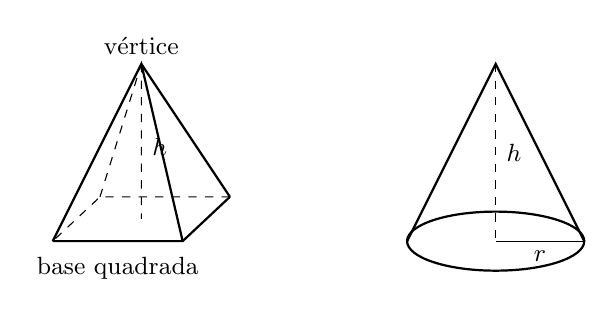
\begin{tikzpicture}[scale=0.75]
  % piramide de base quadrada
  \coordinate (P1) at (-1.3,0);
  \coordinate (P2) at (0.9,0);
  \coordinate (P3) at (1.7,0.75);
  \coordinate (P4) at (-0.5,0.75);
  \coordinate (S) at (0.2,3.0);
  \draw[thick] (P1) -- (P2) -- (P3);
  \draw[dashed] (P3) -- (P4) -- (P1);
  \draw[thick] (P1) -- (S) -- (P2);
  \draw[thick] (P3) -- (S);
  \draw[dashed] (P4) -- (S);
  \draw[dashed] (S) -- (0.2,0.375);
  \node[right, font=\small] at (0.22,1.6) {$h$};
  \node[above, font=\small] at (S) {vértice};
  \node[below, font=\small] at (-0.2,-0.1) {base quadrada};
  % cone
  \begin{scope}[xshift=6.2cm]
  \draw[thick] (0,0) ellipse (1.5 and 0.5);
  \coordinate (T) at (0,3.0);
  \draw[thick] (-1.5,0) -- (T) -- (1.5,0);
  \draw[dashed] (T) -- (0,0);
  \node[right, font=\small] at (0.02,1.5) {$h$};
  \draw[thin] (0,0) -- (1.5,0) node[midway, below, font=\small] {$r$};
  \end{scope}
\end{tikzpicture}

{\small Uma \omterm{def:g8:solids:def}{pirâmide} de base quadrada e um \omterm{def:g8:solids:def}{cone}: uma base poligonal ou
circular, um \omterm{def:g5:solids:def}{vértice} do topo e a altura medida perpendicularmente à
base.}
\end{omfigure}

\begin{example}[Contar faces, arestas e vértices]\label{ex:g8:solids:count}
Uma \omterm{def:g8:solids:def}{pirâmide} de base quadrada tem $5$ \omterm{def:g5:solids:def}{faces} ($1$ quadrado $+ 4$
triângulos), $8$ arestas e $5$ \omterm{def:g5:solids:def}{vértices}. Com uma base de $n$ lados:
$n + 1$ \omterm{def:g5:solids:def}{faces}, $2n$ arestas, $n + 1$ \omterm{def:g5:solids:def}{vértices}. Confira o padrãozinho
de Euler: \omterm{def:g5:solids:def}{faces} $+$ \omterm{def:g5:solids:def}{vértices} $=$ arestas $+ 2$.
\end{example}

\section{Volume}

\begin{theorem}[Volume de uma pirâmide ou de um cone]\label{thm:g8:solids:volume}
Para uma \omterm{def:g8:solids:def}{pirâmide} ou um \omterm{def:g8:solids:def}{cone} de \omterm{def:g6:measure:area}{área} da base $B$ e altura $h$:
\[
V = \frac{1}{3}\, B \times h
\]
--- um terço do \omterm{def:g7:areas:prism}{prisma} ou do \omterm{def:g7:areas:prism}{cilindro} de mesma base e mesma altura.
Para um \omterm{def:g8:solids:def}{cone} de \omterm{def:g3:shapes:shapes}{raio} da base $r$: $V = \frac13 \pi r^2 h$.
\end{theorem}
\admitted

\begin{remark}[Por que um terço?]
Encha de água uma \omterm{def:g8:solids:def}{pirâmide} oca e despeje o conteúdo no \omterm{def:g7:areas:prism}{prisma} de mesma
base e mesma altura: são precisos exatamente três enchimentos. Melhor
ainda: um \omterm{def:g5:solids:def}{cubo} pode ser cortado em três \omterm{def:g8:solids:def}{pirâmides} idênticas, cada uma
com uma \omterm{def:g5:solids:def}{face} do \omterm{def:g5:solids:def}{cubo} como base e um \omterm{def:g5:solids:def}{vértice} do \omterm{def:g5:solids:def}{cubo} como \omterm{def:g5:solids:def}{vértice} do
topo (tente visualizar!). Uma demonstração geral usa a integração, uma
ferramenta do volume do ensino médio.
\end{remark}

\begin{example}\label{ex:g8:solids:volume}
Uma \omterm{def:g8:solids:def}{pirâmide} tem base quadrada de lado $5$ cm e altura $9$ cm:
\begin{enumerate}
  \item \omterm{def:g6:measure:area}{área} da base: $B = 5^2 = 25$ cm$^2$;
  \item \omterm{def:g6:measure:volume}{volume}: $V = \frac13 \times 25 \times 9 = 25 \times 3 = 75$
        cm$^3$.
\end{enumerate}
Uma casquinha de sorvete de \omterm{def:g3:shapes:shapes}{raio} $3$ cm e altura $10$ cm:
\[
V = \frac13 \times \pi \times 3^2 \times 10 = 30\pi \approx 94
\text{ cm}^3 .
\]
\end{example}

\begin{example}[Cuidado com a altura]\label{ex:g8:solids:slant}
Num \omterm{def:g8:solids:def}{cone}, não confunda a altura $h$ (do \omterm{def:g5:solids:def}{vértice} do topo até o centro
da base, perpendicular) com a \emph{geratriz} $s$ (do \omterm{def:g5:solids:def}{vértice} do topo
até a borda). As duas se ligam por Pitágoras
(\cref{thm:g8:pythagoras:direct}) no \omterm{def:g6:shapes:triangles}{triângulo retângulo}
vértice--centro--borda:
\[
s^2 = h^2 + r^2 .
\]
Um \omterm{def:g8:solids:def}{cone} com $r = 3$ e $s = 5$ tem, portanto, altura
$h = \sqrt{25 - 9} = 4$, e \omterm{def:g6:measure:volume}{volume}
$\frac13 \pi \times 9 \times 4 = 12\pi$.
\end{example}

\begin{method}[Problemas de volume]\label{met:g8:solids:method}
\begin{enumerate}
  \item Identifique o \omterm{def:g5:solids:def}{sólido} (\omterm{def:g7:areas:prism}{prisma}/\omterm{def:g7:areas:prism}{cilindro}: $V = Bh$;
        \omterm{def:g8:solids:def}{pirâmide}/\omterm{def:g8:solids:def}{cone}: $V = \frac13 Bh$);
  \item calcule primeiro a \omterm{def:g6:measure:area}{área} da base $B$, como um passo separado;
  \item confira que a altura é perpendicular à base (use Pitágoras se
        a geratriz for dada);
  \item multiplique, mantenha as unidades coerentes e converta no fim,
        se precisar ($1$ L $= 1000$ cm$^3$).
\end{enumerate}
\end{method}

\section{Planificações}

\begin{example}[Planificação de uma pirâmide]\label{ex:g8:solids:net}
Desdobrar uma \omterm{def:g8:solids:def}{pirâmide} regular de base quadrada a achata na
\emph{\omterm{def:g5:solids:net}{planificação}} dela: a base quadrada com quatro \omterm{def:g6:shapes:triangles}{triângulos
isósceles} idênticos presos aos lados. Os lados iguais desses
triângulos são as \emph{arestas laterais} da \omterm{def:g8:solids:def}{pirâmide} --- o
comprimento deles não é nem $h$ nem a altura de uma \omterm{def:g5:solids:def}{face}, então marque
tudo com cuidado antes de cortar o papelão.
\end{example}

\begin{omfigure}
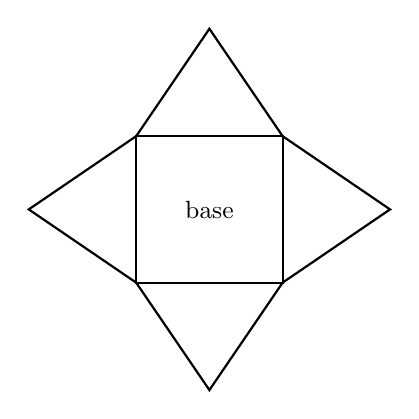
\begin{tikzpicture}[scale=0.62]
  \draw[thick] (0,0) rectangle (3,3);
  \draw[thick] (0,0) -- (1.5,-2.2) -- (3,0);
  \draw[thick] (3,0) -- (5.2,1.5) -- (3,3);
  \draw[thick] (0,3) -- (1.5,5.2) -- (3,3);
  \draw[thick] (0,0) -- (-2.2,1.5) -- (0,3);
  \node[font=\small] at (1.5,1.5) {base};
\end{tikzpicture}

{\small A \omterm{def:g5:solids:net}{planificação} de uma \omterm{def:g8:solids:def}{pirâmide} de base quadrada: dobre os
quatro triângulos para cima até as pontas se encontrarem.}
\end{omfigure}

\section{Exercícios}

\begin{exercise}[$\star$]\label{exo:g8:solids:1}
Quantas \omterm{def:g5:solids:def}{faces}, arestas e \omterm{def:g5:solids:def}{vértices} tem uma \omterm{def:g8:solids:def}{pirâmide} de base triangular
(um \emph{tetraedro})? E uma de base hexagonal?
\end{exercise}

\begin{exercise}[$\star$]\label{exo:g8:solids:2}
Calcule o \omterm{def:g6:measure:volume}{volume} de uma \omterm{def:g8:solids:def}{pirâmide} de \omterm{def:g6:measure:area}{área} da base $36$ cm$^2$ e altura
$10$ cm; e o de uma \omterm{def:g8:solids:def}{pirâmide} de base retangular $6 \times 4$ cm e
altura $7.5$ cm.
\end{exercise}

\begin{exercise}[$\star$]\label{exo:g8:solids:3}
Calcule o \omterm{def:g6:measure:volume}{volume} de um \omterm{def:g8:solids:def}{cone} de \omterm{def:g3:shapes:shapes}{raio} $5$ cm e altura $9$ cm (exato, com
$\pi$, e depois arredondado ao cm$^3$).
\end{exercise}

\begin{exercise}[$\star$]\label{exo:g8:solids:4}
Um \omterm{def:g7:areas:prism}{cilindro} e um \omterm{def:g8:solids:def}{cone} têm o mesmo \omterm{def:g3:shapes:shapes}{raio} $4$ cm e a mesma altura $12$
cm. Calcule os dois \omterm{def:g6:measure:volume}{volumes}. Qual é a razão entre eles?
\end{exercise}

\begin{exercise}[$\star$]\label{exo:g8:solids:5}
Uma \omterm{def:g8:solids:def}{pirâmide} tem \omterm{def:g6:measure:volume}{volume} $56$ cm$^3$ e altura $8$ cm. Qual é a \omterm{def:g6:measure:area}{área} da
base dela? (Escreva a fórmula do \omterm{def:g6:measure:volume}{volume} e resolva.)
\end{exercise}

\begin{exercise}[$\star$]\label{exo:g8:solids:6}
Esboce a \omterm{def:g5:solids:net}{planificação} de um \omterm{def:g8:solids:def}{cone} (um disco para a base e um setor de
um disco maior para a superfície lateral). Qual medida do \omterm{def:g8:solids:def}{cone} é o
\omterm{def:g3:shapes:shapes}{raio} desse setor: a altura $h$ ou a geratriz $s$?
\end{exercise}

\begin{exercise}[$\star\star$]\label{exo:g8:solids:7}
A \omterm{def:g8:solids:def}{pirâmide} do Louvre tem base quadrada de lado aproximadamente $35$ m
e altura de cerca de $22$ m. Estime o \omterm{def:g6:measure:volume}{volume} dela, arredondando à
centena de metros cúbicos.
\end{exercise}

\begin{exercise}[$\star\star$]\label{exo:g8:solids:8}
Um \omterm{def:g8:solids:def}{cone} tem geratriz $13$ cm e \omterm{def:g3:shapes:shapes}{raio} da base $5$ cm. Calcule a altura
dele e depois o \omterm{def:g6:measure:volume}{volume} (exato, com $\pi$).
\end{exercise}

\begin{exercise}[$\star\star$]\label{exo:g8:solids:9}
Uma taça cônica de \omterm{def:g3:shapes:shapes}{raio} $4$ cm e altura $9$ cm é enchida até a borda e
depois despejada num copo cilíndrico de \omterm{def:g3:shapes:shapes}{raio} $4$ cm. Que altura o
líquido alcança no \omterm{def:g7:areas:prism}{cilindro}?
\end{exercise}

\begin{exercise}[$\star\star$]\label{exo:g8:solids:10}
Uma ampulheta é feita de dois \omterm{def:g8:solids:def}{cones} idênticos (\omterm{def:g3:shapes:shapes}{raio} $2$ cm, altura
$4.5$ cm) unidos pelas pontas. Toda a areia enche exatamente um \omterm{def:g8:solids:def}{cone}.
Calcule o \omterm{def:g6:measure:volume}{volume} de areia (exato e depois em cm$^3$ arredondado ao
décimo) e a \omterm{def:g6:fractions:def}{fração} do \omterm{def:g6:measure:volume}{volume} interno total da ampulheta que a areia
ocupa.
\end{exercise}

\begin{exercise}[$\star\star\star$]\label{exo:g8:solids:11}
Uma \omterm{def:g8:solids:def}{pirâmide} de base quadrada de lado $6$ cm tem o \omterm{def:g5:solids:def}{vértice} do topo
diretamente acima de um canto da base, à altura $8$ cm.
\begin{enumerate}
  \item A fórmula $V = \frac13 Bh$ continua valendo? (Continua --- o
        \omterm{def:g5:solids:def}{vértice} do topo não precisa ficar centrado. Calcule $V$.)
  \item Calcule o comprimento da aresta lateral mais longa, do \omterm{def:g5:solids:def}{vértice}
        do topo até o canto oposto da base (dois passos de Pitágoras:
        primeiro a diagonal da base).
\end{enumerate}
\end{exercise}

\section{Problema: um cubo cortado em três pirâmides}

\begin{problem}[{Problema de fim de semana --- de onde vem o fator
$\frac13$, e o que acontece com uma pirâmide cortada na metade da
altura}]
\label{pb:g8:solids:1}
A observação depois do \cref{thm:g8:solids:volume} afirma que um \omterm{def:g5:solids:def}{cubo}
pode ser cortado em três \omterm{def:g8:solids:def}{pirâmides} idênticas --- ``tente
visualizar!''. Este problema visualiza isso com precisão, tira daí o
famoso fator $\frac13$ de modo honesto, depois corta o \omterm{def:g5:solids:def}{cubo} de um
segundo jeito, em \emph{seis} \omterm{def:g8:solids:def}{pirâmides}, e termina fatiando uma
\omterm{def:g8:solids:def}{pirâmide} na \omterm{def:g3:division:half}{metade} da altura dela --- com um resultado que poucas
pessoas acertam na primeira tentativa.

Em todo o problema, $ABCDEFGH$ é um \omterm{def:g5:solids:def}{cubo} de lado $a$: base $ABCD$,
\omterm{def:g5:solids:def}{face} de cima $EFGH$, com $E$ acima de $A$, $F$ acima de $B$, $G$ acima
de $C$ e $H$ acima de $D$.

\medskip
\noindent\textbf{Parte I --- Três \omterm{def:g8:solids:def}{pirâmides} com o mesmo \omterm{def:g5:solids:def}{vértice}.}
\begin{enumerate}
  \item O \omterm{def:g5:solids:def}{vértice} $G$ pertence a três \omterm{def:g5:solids:def}{faces} do \omterm{def:g5:solids:def}{cubo}. Liste as três
        \omterm{def:g5:solids:def}{faces} que \emph{não} contêm $G$ e descreva as três \omterm{def:g8:solids:def}{pirâmides}
        obtidas tomando cada uma delas como base, sempre com o
        \omterm{def:g5:solids:def}{vértice} $G$ no topo. Quantas \omterm{def:g5:solids:def}{faces}, arestas e \omterm{def:g5:solids:def}{vértices} tem
        cada \omterm{def:g8:solids:def}{pirâmide} (\cref{ex:g8:solids:count})?
  \item Explique por que girar o \omterm{def:g5:solids:def}{cubo} de um terço de volta em torno da
        diagonal longa $(AG)$ deixa o \omterm{def:g5:solids:def}{cubo} inalterado, mas embaralha
        em ciclo as três bases da questão 1 --- e por que as três
        \omterm{def:g8:solids:def}{pirâmides} são, portanto, cópias idênticas umas das outras.
  \item Admitindo que as três \omterm{def:g8:solids:def}{pirâmides} preenchem o \omterm{def:g5:solids:def}{cubo} sem se
        sobrepor (um modelo de papelão é bem convincente), deduza o
        \omterm{def:g6:measure:volume}{volume} de cada uma.
  \item Confira isso com a fórmula do \cref{thm:g8:solids:volume}: a
        \omterm{def:g8:solids:def}{pirâmide} de base $ABCD$ e \omterm{def:g5:solids:def}{vértice} $G$ tem o \omterm{def:g5:solids:def}{vértice} do topo
        diretamente acima de um \emph{canto} da base dela, exatamente
        como no \cref{exo:g8:solids:11}. Identifique a altura dela,
        aplique a fórmula e compare.
  \item Para um \omterm{def:g5:solids:def}{cubo} de lado $6$ cm, dê o \omterm{def:g6:measure:volume}{volume} de cada uma das três
        \omterm{def:g8:solids:def}{pirâmides} --- e explique o que essa decomposição tem a ver com
        a experiência de despejar água do capítulo (três enchimentos
        da \omterm{def:g8:solids:def}{pirâmide} para um \omterm{def:g7:areas:prism}{prisma}).
\end{enumerate}

\medskip
\noindent\textbf{Parte II --- Seis \omterm{def:g8:solids:def}{pirâmides} com o mesmo centro.}
Agora seja $O$ o centro do \omterm{def:g5:solids:def}{cubo}, e ligue $O$ aos quatro \omterm{def:g5:solids:def}{vértices} de
cada uma das seis \omterm{def:g5:solids:def}{faces}.
\begin{enumerate}[resume]
  \item Descreva as seis \omterm{def:g8:solids:def}{pirâmides} obtidas e explique por que elas são
        cópias idênticas umas das outras. Qual é a altura de cada uma?
  \item Deduza, repartindo o \omterm{def:g6:measure:volume}{volume} do \omterm{def:g5:solids:def}{cubo}, o \omterm{def:g6:measure:volume}{volume} de cada uma das
        seis \omterm{def:g8:solids:def}{pirâmides}.
  \item Recalcule esse \omterm{def:g6:measure:volume}{volume} com a fórmula $V = \frac13 B h$ e
        verifique que as duas respostas concordam.
  \item As duas decomposições confirmam o fator $\frac13$ para umas
        \omterm{def:g8:solids:def}{pirâmides} bem especiais. Explique por que elas ainda não
        \emph{demonstram} o \cref{thm:g8:solids:volume} para toda
        \omterm{def:g8:solids:def}{pirâmide} e todo \omterm{def:g8:solids:def}{cone} --- e diga como o capítulo lida com essa
        lacuna: que enunciado é admitido, que experiência o apoia e em
        que volume da série ele é demonstrado com honestidade.
  \item Um \omterm{def:g5:solids:def}{cubo} de lado $6$ cm é cortado nas seis \omterm{def:g8:solids:def}{pirâmides} do centro.
        Calcule o \omterm{def:g6:measure:volume}{volume} de cada uma, pelos dois caminhos.
\end{enumerate}

\medskip
\noindent\textbf{Parte III --- Cortar uma \omterm{def:g8:solids:def}{pirâmide} na \omterm{def:g3:division:half}{metade} da
altura.}
$SABCD$ é uma \omterm{def:g8:solids:def}{pirâmide} regular de base quadrada: lado da base $c$,
altura $h$, \omterm{def:g5:solids:def}{vértice} $S$ acima do centro da base. Corte-a pelo plano que
passa pelos \emph{pontos médios} das quatro arestas laterais $[SA]$,
$[SB]$, $[SC]$, $[SD]$.
\begin{enumerate}[resume]
  \item Aplique o teorema dos pontos médios
        (\cref{thm:g8:midpoints:direct}) no triângulo $SAB$: qual é a
        direção e qual é o comprimento do \omterm{def:g6:lines:objects}{segmento} que liga os pontos
        médios de $[SA]$ e $[SB]$? Deduza que o corte é um quadrado de
        lado $\frac{c}{2}$, paralelo à base, à altura $\frac{h}{2}$.
  \item A peça acima do corte é ela mesma uma \omterm{def:g8:solids:def}{pirâmide} de base
        quadrada. Dê o lado da base e a altura dela, e mostre que o
        \omterm{def:g6:measure:volume}{volume} dela é exatamente \emph{um oitavo} do \omterm{def:g6:measure:volume}{volume} original
        $V$.
  \item Deduza o \omterm{def:g6:measure:volume}{volume} da peça de baixo (o \emph{tronco}, a forma de
        uma \omterm{def:g8:solids:def}{pirâmide} inacabada). Em que razão o corte na \omterm{def:g3:division:half}{metade} da
        altura reparte o \omterm{def:g6:measure:volume}{volume}?
  \item A \omterm{def:g8:solids:def}{pirâmide} do Louvre (\cref{exo:g8:solids:7}: lado da base
        $35$ m, altura $22$ m) é limpa em duas campanhas: primeiro o
        vidro acima da \omterm{def:g3:division:half}{metade} da altura e depois o vidro abaixo dela.
        Que \omterm{def:g6:fractions:def}{fração} do \emph{\omterm{def:g6:measure:volume}{volume}} fica abaixo da \omterm{def:g3:division:half}{metade} da altura?
        Estime-a em metros cúbicos, arredondando à centena.
  \item A moral geral: se \emph{todas} as dimensões de uma \omterm{def:g8:solids:def}{pirâmide}
        forem multiplicadas por $2$, o que acontece com o \omterm{def:g6:measure:volume}{volume} dela?
        Por que fator o \omterm{def:g6:measure:volume}{volume} cresce quando cada dimensão é
        multiplicada por $k$ --- e como isso explica, em uma linha, o
        ``um oitavo'' da questão 12?
\end{enumerate}
\end{problem}
